\subsection{UI feedback}
Although the basic functionality is provided, the look and feel of the application in no way matches the mockups and descriptions included in the documentation. It is clear the development effort was put into other parts of the system.

As an example, we can see below a comparison of the sign up screen in the mockup and in the final prototype:
\begin{figure}[H]
    \centering
    \begin{minipage}{.4\textwidth}
        \centering
        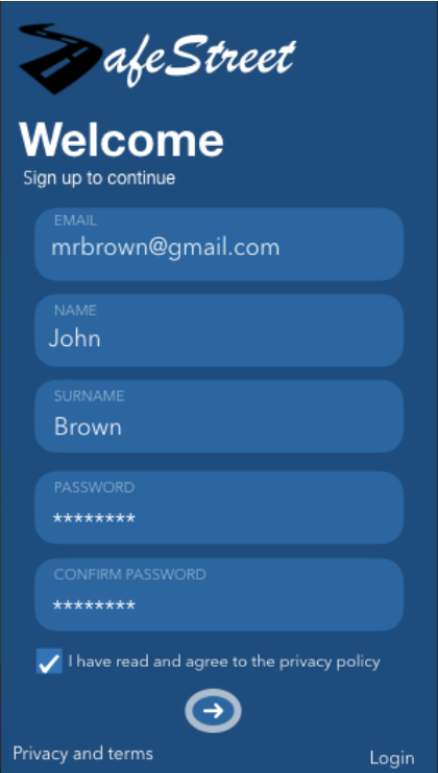
\includegraphics[width=.8\textwidth]{Images/mockup-sign-up.png}
        \caption{\label{fig:mockup-sign-up}Mockup - Sign up.}
    \end{minipage}
    \begin{minipage}{.422\textwidth}
        \centering
        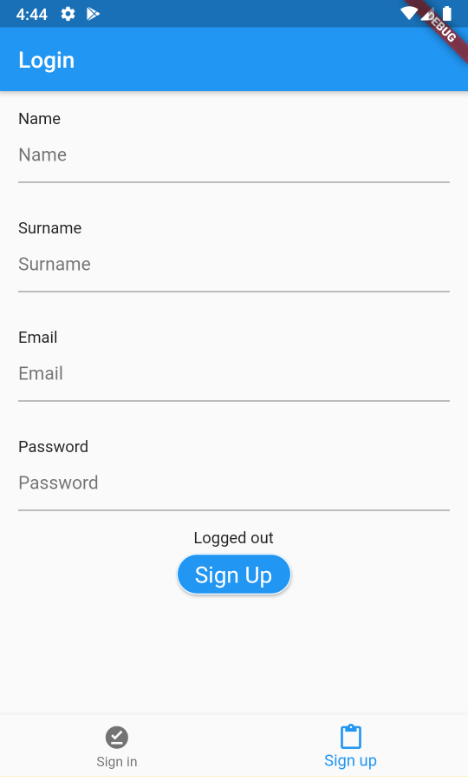
\includegraphics[width=.8\textwidth]{Images/prototype-sign-up.png}
        \caption{\label{fig:prototype-sign-up}Prototype - Sign up.}
    \end{minipage}
    \end{figure}

\subsection{Version differences}
Disregarding the differences with the mockup, the installation process chosen results in different UIs and functionality for the app.

\begin{figure}[H]
    \centering
    \begin{minipage}{.4\textwidth}
        \centering
        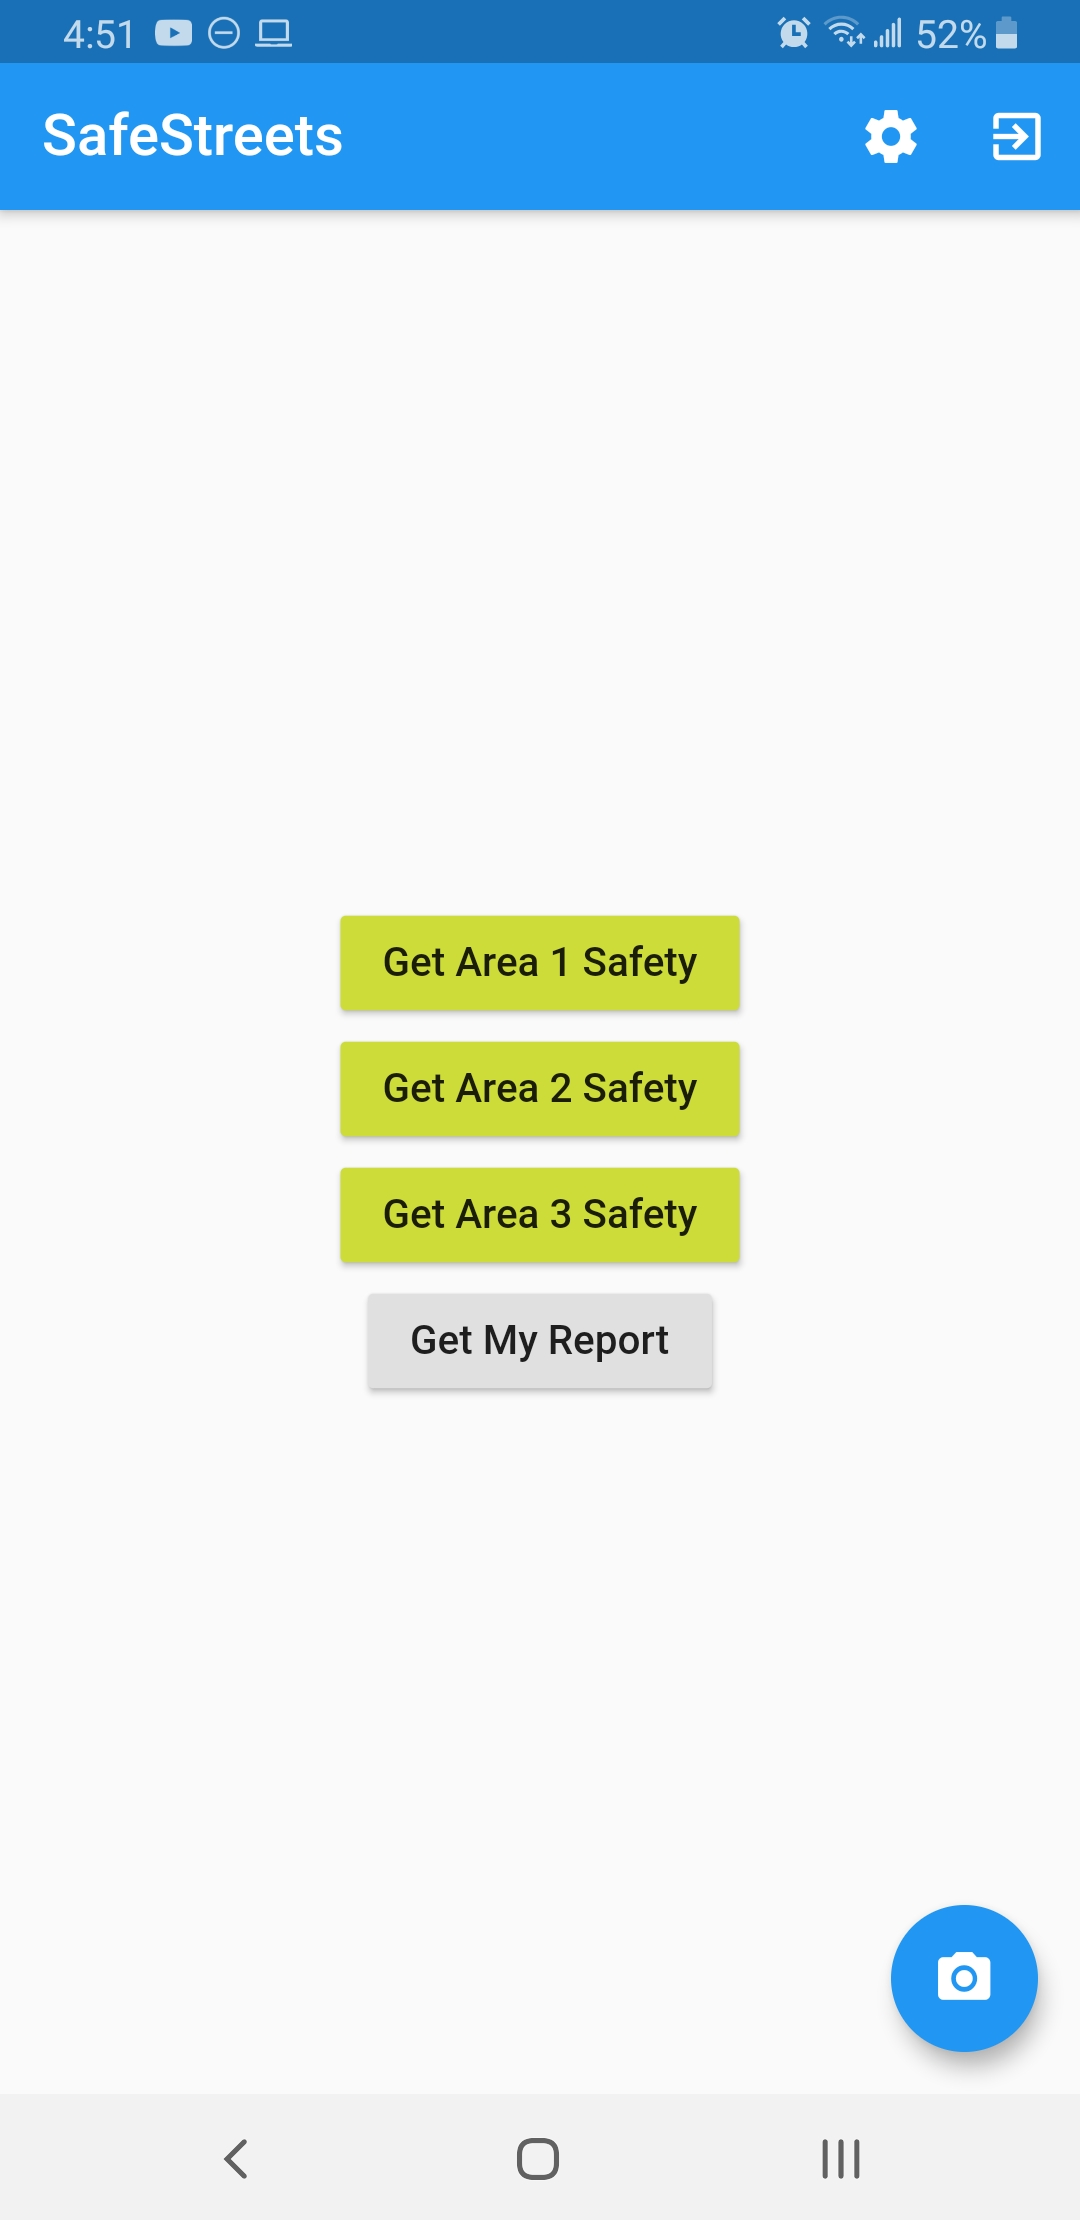
\includegraphics[width=.8\textwidth]{Images/store-home.jpg}
        \caption{\label{fig:store-home}Play store app - Home screen.}
    \end{minipage}
    \begin{minipage}{.465\textwidth}
        \centering
        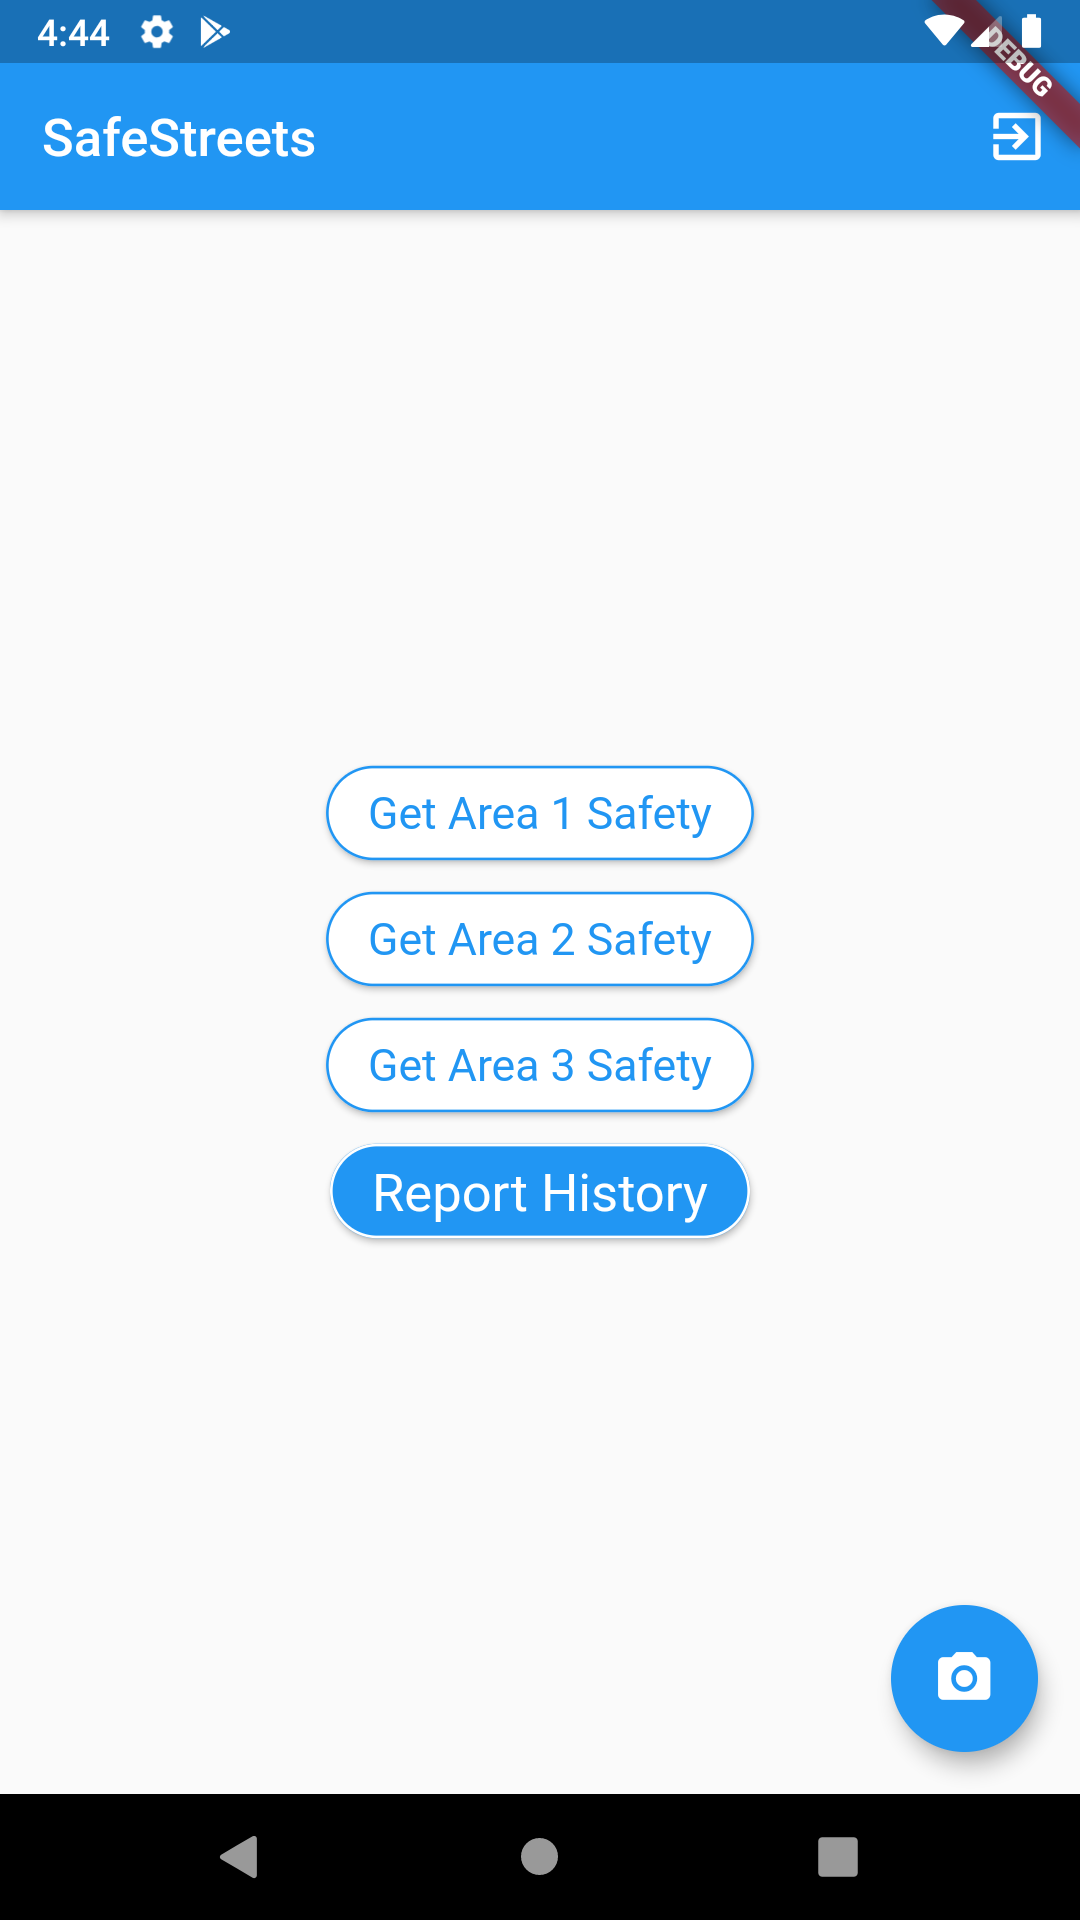
\includegraphics[width=.8\textwidth]{Images/source-home.png}
        \caption{\label{fig:source-home}Source code - Home screen.}
    \end{minipage}
    \end{figure}

As seen in the figures, the button design is different. Moreover, when running the app from the source code there is no settings button to enable notifications.

\subsection{Documentation inconsistencies}
As seen in the UI feedback section, there are inconsistencies between the RASD and what is implemented. In addition, multiple key use cases are missing, namely the area safety functionality for users, and interventions suggestion and validation of reports for authorities.
Finally, as mentioned in the acceptance tests section, the notification functionality, which should only we accessible to authorities, is also present when logged in as a regular user.